
\section{Analysis of volcanic earthquakes} 
\label{sect:volcanic}

SEISAN is often used for volcanic monitoring. Many of the standard tools used 
in SEISAN can also be used for volcanic earthquakes, like epicenter 
location and magnitude. However, more special tool are also needed 
and below there is a description how this is done at the British Geological Survey (BGS).

Another description, made by Andrew Lockhart at the USGS, is given 
in a separate manual (\texttt{seisan\_volcano.pdf} in INF or at 
\url{http://seis.geus.net/software/seisan/seisan\_volcano.pdf}
). 
This manual is a mini SEISAN manual detailing the steps under Windows.

\textbf{Volcano monitoring at BGS}

By \textbf{Brian Baptie} 

\textbf{Background}

An important part of volcanic seismology and the seismic monitoring of active volcanoes is the correct recognition of the different types of seismic event generated by the volcanic activity. The principal event types include, volcano-tectonic events, caused by shear or tensile failure of rocks; long period events, generated by a volumetric source in a liquid; hybrid events; and volcanic tremor.  

To be of value for volcanic monitoring, any database of seismic events should include the type or sub-class of individual events. This should allow users to then extract phase and location information over a selected time period for individual event types and calculate hourly and daily rates of event. Simple histogram plots showing the distribution of subclasses over time can be generated with the program VOLCSTAT\index{VOLCSTAT} (Unix only). 

Initialization 

\index{VOLCANO.DEF}
The user should create a text file in the DAT directory called \texttt{VOLCANO.DEF} 
(an example is already in the directory). The format of this file will 
be one line of text (80A) followed by successive lines with the 
format "i2,1x,6A,1X,40a" for number, sub-class code and description. 
An example of the file is shown below. Comments are preceded with '!'. 

\index{Volcanic tremor}\index{Format, volcanic information}
\begin{verbatim}
Current volcano sub-classes:   ! Comment line 80 characters 
1  vt     volcano-tectonic     ! Individual sub-class line 
2  hybrid hybrid
3  lp     long-period
4  tremor volcanic tremor 
5  rf     rockfall 
6  un     unknown 
7         QUIT                 ! The last line should contain 
                                 this entry
\end{verbatim}

Registering volcanic sub-classes 

Registration should be carried out as normal in MULPLT. From multi-trace mode enter 'p' to create a new s-file for the event in the database. Answering 'LV' to the prompt for event type marks the event as a local volcanic in the headers. If the \texttt{VOLCANO.DEF} file has been set up correctly in the DAT directory, the information on the different sub-classes will be printed to the terminal. Choosing an appropriate number selects the volcanic sub-class. The sub-class code is then entered in the s-file. 

Modification of the s-file to incorporate volcanic sub-classes 

The volcanic sub-class information is stored in a type 3 line within the s-file, e.g. 

\begin{verbatim}
 VOLC MAIN tremor 3 

Columns 2:10  'VOLC MAIN'    : Header identifier 
Columns 12:17    a6          : Sub-class flag
Column  80       '3'         : line type identifier 
\end{verbatim}

This allows the use of a maximum 6-character sub-class identifier, e.g. 'hybrid', which can then be searched for and selected. 

VOLCSTAT\index{VOLCSTAT}: Creating histogram plots 

The program reads S-files directly from the database, and creates 
input files as well as a GMT\index{GMT} script to produce histogram 
plots of the distribution of subclasses over time. The user needs 
to enter database name, start and end time, and the subclasses that 
are to be plotted. 
An example of a plot is shown in Figure 
\ref{fig:volcstat}.
The program supports 1-char subclass names only.

The following output files are created:

\texttt{volcstat.batch} - c-shell script to generate Postscript output using GMT	\newline
\texttt{volcstat\_counts.ps} - Postscript output file\newline
\texttt{volcstat\_counts\_$<$type$>$.out} - for each event, the Julian date is written out, one file per subclass\newline
\texttt{volcstat\_daily\_$<$type$>$.out} - number of events per day, files written for each subclass\newline
\texttt{volcstat\_counts\_total.out} - total event counts for each subclass\newline

\begin{figure}
\htmlimage{scale=2.0}
\centerline{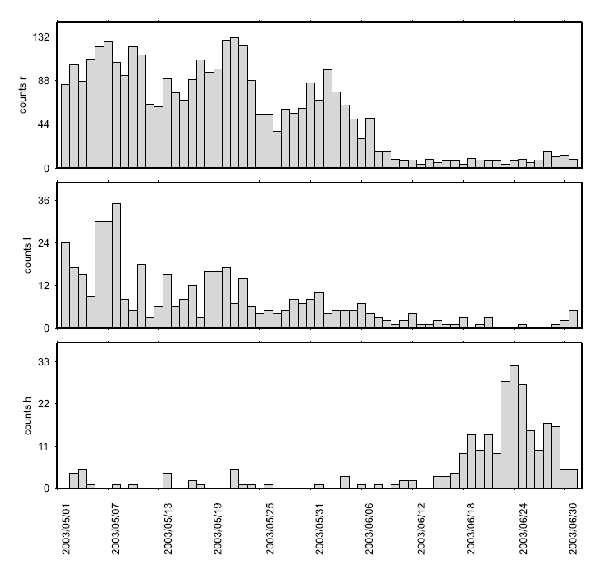
\includegraphics[width=0.9\linewidth]{fig/fig46}}
\caption{Bar diagrams showing distribution of events of different subclasses over time.}
\label{fig:volcstat}
\end{figure}

RSAM

1-minute RSAM data can be created with WAVETOOL.

Future Extensions:\newline
It is intended that additional parameters can be included in the above structure to included 
routine measurements of the volcanic earthquakes. For example, signal duration, peak amplitude 
and mean frequency can be calculated for individual stations and included on additional type 3 
lines with a volcanic identifier. Parameters on each channel can then be averaged an inserted 
on the volcanic header line.

The proposed format for these lines is as follows 

\verbatiminput{include/volc.ext}

This method of inclusion of volcanic parameters should allow for future flexibility such as incorporation of an additional parameter fields in columns 66 to 79. Also the use of type 3 lines means that existing software, such as the update program, are unaffected by these lines. 

